\documentclass[tikz,convert={density=150,size=600,outext=.png}]{standalone}
\usetikzlibrary{shapes, calc, arrows, fit, positioning, decorations, patterns, decorations.pathreplacing, chains, snakes}

\begin{document}
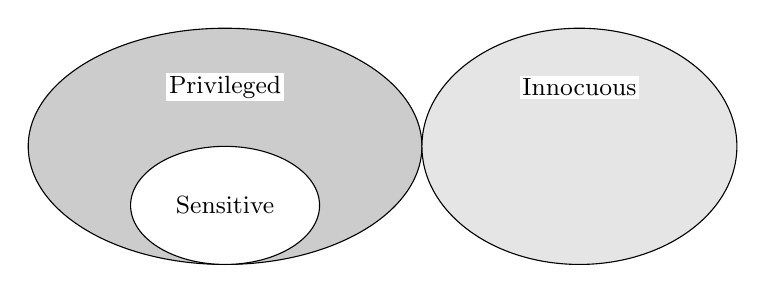
\begin{tikzpicture}[font=\small]
    \fill[draw, fill=black!20] (0,0) circle [x radius=2.5cm, y radius=1.5cm];
    \fill[draw, fill=black!10] (4.5,0) circle [x radius=2cm, y radius=1.5cm];
    \node[fill=white, inner sep=1pt] at (0.0,0.75) {Privileged};
    \node[fill=white, inner sep=1pt] at (4.5,0.75) {Innocuous};
    
    \fill[draw, fill=white] (0,-0.75) circle [x radius=1.2cm, y radius=0.75cm];
    \node[fill=white, inner sep=1pt] at (0,-0.75) {Sensitive};
\end{tikzpicture}
\end{document}
